%Theory behind RNN
%lstm as improvement on rnn
%Theory of lstm, inner workings
%Use of hidden layers
Typical neural networks do not have a state that allows them to "remember" previous data points, for prediction. This is where the basic idea behind a recurrent neural network (RNN for short) comes from. It has a hidden state representing its memory regarding previous data. It will then be able to make decisions regarding new data, taking this previous data into account.

If we take a look at the sentences below, the idea is that the RNN would first be able to understand the nearby context; that the next word is supposed to be a reason for staying home. And also understand the larger context, (that the pandemic is that reason) without needing to remember unnecessary stuff like the words "is", "a" and so on. It should then be able to predict that pandemic would be the next word in the sentence.

\begin{itemize}
	\item There is a pandemic. I had to stay home from university because of the \_\_\_
\end{itemize}

RNNs are extremely flexible in how they can be used. There are, in fact, four main ways they transform the input into something usable. 

The first is in a "one to many" fashion, in which they take a single input and output a sequence. This could be useful for tasks like generating descriptions based on fixed size inputs such as images. 

The second is in a "many to one" fashion in which the input is a sequence, and the network outputs a single result a the end. This is useful in cases where an entire sequence has a single class to be predicted.

The last two both output in a "many to many" fashion, but how they do it is significantly different. The first case outputs a completely new sequence that is not neccesarily the same length as the input sequence, after having seen the entire input. This is useful for networks trying to represent the data in a different way. The last case is the one that will be described further down in this report. This case outputs an element of a new sequence for each element in the input. This means that for each output element, the RNN only knows about previous elements. This makes it the perfect candidate for next token prediction.

\begin{figure}[h]
	\centering
		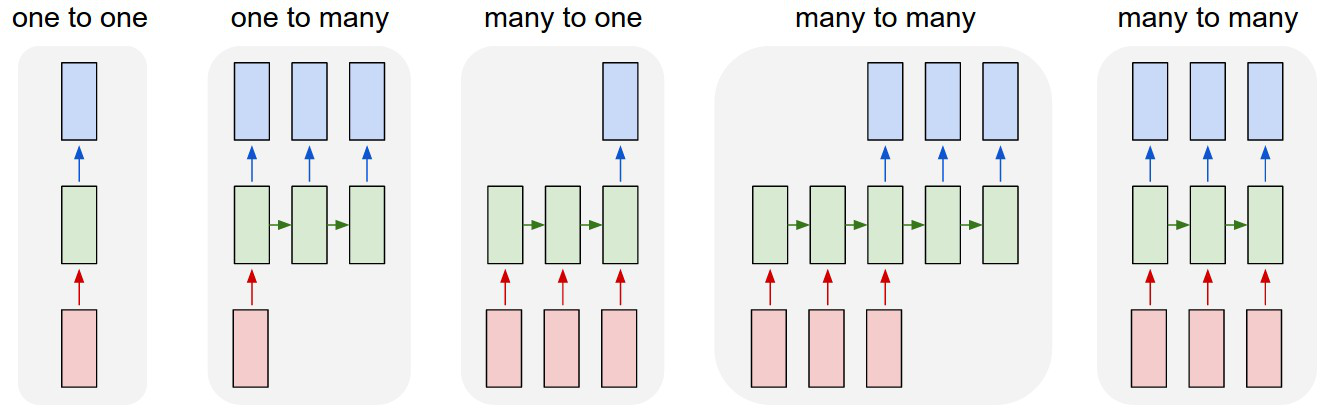
\includegraphics[width=0.5\textwidth]{latex/IMGs/rnn_types.png}}
  	\caption{A visual representation of the output types described. Image Source:\cite{rnn}}
\end{figure}

The basic structure of an RNN is quite simple, consisting of a single linear layer and activation function, which is usually the $tanh$ function. The network is interesting in that each "cell" passes along a hidden state as input to the next cell. This means that each cell takes both the current input element and the previous cell's output and concatenates them and uses this as input to the linear layer.

\begin{figure}[h]
	\centering
		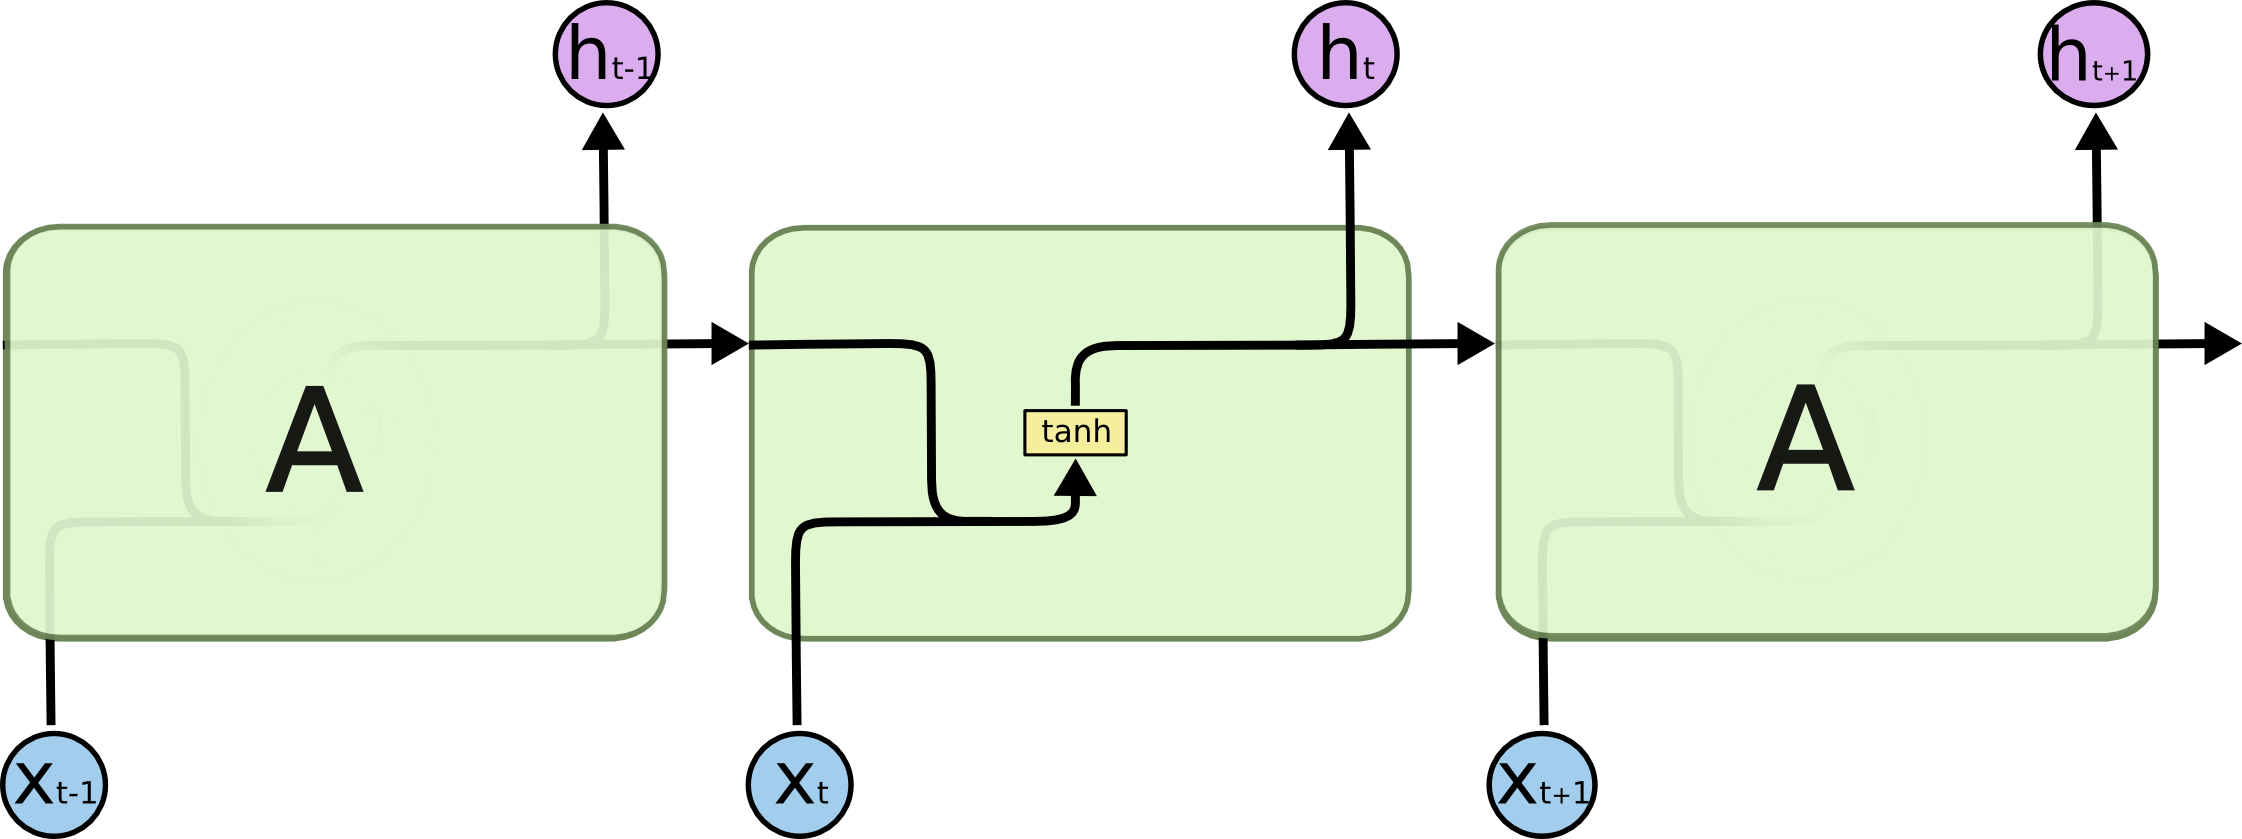
\includegraphics[width=0.5\textwidth]{latex/IMGs/rnn.png}}
  	\caption{A visual representation of the inner structure of an RNN. Image Source:\cite{rnn}}
\end{figure}

\subsubsection{The exploding/vanishing gradient problem}
One major issue with using basic RNNs is the fact that they suffer quite heavily from the exploding/vanishing gradient problem. This problem arises from the fact that very large gradients and gradients very close to zero tend to approach infinity and zero respectively, as they are multiplied together during backpropagation.

To show this, let's consider the following example. The gradient when using the backprop through time algorithm looks as follows:
